% Options for packages loaded elsewhere
\PassOptionsToPackage{unicode}{hyperref}
\PassOptionsToPackage{hyphens}{url}
\PassOptionsToPackage{dvipsnames,svgnames*,x11names*}{xcolor}
%
\documentclass[
]{article}
\usepackage{lmodern}
\usepackage{amssymb,amsmath}
\usepackage{ifxetex,ifluatex}
\ifnum 0\ifxetex 1\fi\ifluatex 1\fi=0 % if pdftex
  \usepackage[T1]{fontenc}
  \usepackage[utf8]{inputenc}
  \usepackage{textcomp} % provide euro and other symbols
\else % if luatex or xetex
  \usepackage{unicode-math}
  \defaultfontfeatures{Scale=MatchLowercase}
  \defaultfontfeatures[\rmfamily]{Ligatures=TeX,Scale=1}
  \setmonofont[Scale=0.7]{Source Code Pro}
\fi
% Use upquote if available, for straight quotes in verbatim environments
\IfFileExists{upquote.sty}{\usepackage{upquote}}{}
\IfFileExists{microtype.sty}{% use microtype if available
  \usepackage[]{microtype}
  \UseMicrotypeSet[protrusion]{basicmath} % disable protrusion for tt fonts
}{}
\makeatletter
\@ifundefined{KOMAClassName}{% if non-KOMA class
  \IfFileExists{parskip.sty}{%
    \usepackage{parskip}
  }{% else
    \setlength{\parindent}{0pt}
    \setlength{\parskip}{6pt plus 2pt minus 1pt}}
}{% if KOMA class
  \KOMAoptions{parskip=half}}
\makeatother
\usepackage{xcolor}
\IfFileExists{xurl.sty}{\usepackage{xurl}}{} % add URL line breaks if available
\IfFileExists{bookmark.sty}{\usepackage{bookmark}}{\usepackage{hyperref}}
\hypersetup{
  pdftitle={ANS performance briefing - Germany},
  pdfauthor={EUROCONTROL Performance Review Unit},
  colorlinks=true,
  linkcolor=Maroon,
  filecolor=Maroon,
  citecolor=Blue,
  urlcolor=blue,
  pdfcreator={LaTeX via pandoc}}
\urlstyle{same} % disable monospaced font for URLs
\usepackage[margin=1in]{geometry}
\usepackage{longtable,booktabs}
% Correct order of tables after \paragraph or \subparagraph
\usepackage{etoolbox}
\makeatletter
\patchcmd\longtable{\par}{\if@noskipsec\mbox{}\fi\par}{}{}
\makeatother
% Allow footnotes in longtable head/foot
\IfFileExists{footnotehyper.sty}{\usepackage{footnotehyper}}{\usepackage{footnote}}
\makesavenoteenv{longtable}
\usepackage{graphicx,grffile}
\makeatletter
\def\maxwidth{\ifdim\Gin@nat@width>\linewidth\linewidth\else\Gin@nat@width\fi}
\def\maxheight{\ifdim\Gin@nat@height>\textheight\textheight\else\Gin@nat@height\fi}
\makeatother
% Scale images if necessary, so that they will not overflow the page
% margins by default, and it is still possible to overwrite the defaults
% using explicit options in \includegraphics[width, height, ...]{}
\setkeys{Gin}{width=\maxwidth,height=\maxheight,keepaspectratio}
% Set default figure placement to htbp
\makeatletter
\def\fps@figure{htbp}
\makeatother
\setlength{\emergencystretch}{3em} % prevent overfull lines
\providecommand{\tightlist}{%
  \setlength{\itemsep}{0pt}\setlength{\parskip}{0pt}}
\setcounter{secnumdepth}{5}
\usepackage{float}
\floatplacement{figure}{H}
\usepackage[table]{xcolor}
% https://github.com/rstudio/rmarkdown/issues/337
\let\rmarkdownfootnote\footnote%
\def\footnote{\protect\rmarkdownfootnote}

% https://github.com/rstudio/rmarkdown/pull/252
\usepackage{titling}
\setlength{\droptitle}{-2em}

\pretitle{\vspace{\droptitle}\centering\huge}
\posttitle{\par}

\preauthor{\centering\large\emph}
\postauthor{\par}

\predate{\centering\large\emph}
\postdate{\par}

\title{ANS performance briefing - Germany}
\author{EUROCONTROL Performance Review Unit}
\date{06/Dec/2019}

\begin{document}
\maketitle

\begin{center}
\includegraphics[width=\textwidth]{images/logo} \end{center}

\newpage

\hypertarget{preface}{%
\section*{Preface}\label{preface}}
\addcontentsline{toc}{section}{Preface}

This performance briefing has been prepared by the EUROCONTROL Performance Review Unit (PRU) in the interest of the exchange of information.

If you have any questions related to this document or if we can help with any ANS performance related matter, then please do not hesitate to contact us: \href{mailto:pru-support@eurocontrol.int}{\nolinkurl{pru-support@eurocontrol.int}}

The information may be copied in whole or in part providing that the copyright notice and disclaimer are included.

The views expressed herein do not necessarily reflect the official views or policy of EUROCONTROL, which makes no warranty, either implied or express, for the information contained in this document, neither does it assume any legal liability or responsibility for the accuracy, completeness or usefulness of this information.

\newpage

\hypertarget{key-observations}{%
\section*{Key observations}\label{key-observations}}
\addcontentsline{toc}{section}{Key observations}

TRAFFIC

\begin{itemize}
\item
  Following the high traffic increase already in 2017 ..
\item
  The strong growth ..
\item
  As a result ..
\end{itemize}

SAFETY

\begin{itemize}
\tightlist
\item
  No data available
\end{itemize}

CAPACITY

En-route ATFM delays

\begin{itemize}
\tightlist
\item
  No en-route ATFM delay..
\end{itemize}

Airport arrival ATFM delays

\begin{itemize}
\tightlist
\item
  No airport arrival ATFM delay..
\end{itemize}

ENVIRONMENT

Horizontal en-route flight efficiency

\begin{itemize}
\tightlist
\item
  In 2008, Finland..
\end{itemize}

Vertical en-route flight efficiency

Vertical flight efficiency during climb and descent

COST-EFFECTIVENESS

\begin{itemize}
\item
  ARMATS represents.. see {[}\protect\hyperlink{ref-pru:ace-report-2015}{1}{]}
\item
  Since ARMATS did not..
\item
  Compared to the..
\end{itemize}

\newpage

% Trigger ToC creation in LaTeX
\tableofcontents

\newpage

\listoffigures

\newpage

\hypertarget{institutional-arrangements}{%
\section{Institutional arrangements}\label{institutional-arrangements}}

\newpage

\hypertarget{traffic-characteristics}{%
\section{Traffic characteristics}\label{traffic-characteristics}}

Sources: NM; STATFOR{[}\protect\hyperlink{ref-7year-forecast-2019}{2}{]}; PRU ANS Performance Data Portal {[}\protect\hyperlink{ref-ANS-perf-data-portal}{3}{]}; CRCO Service Unit Dashboard {[}\protect\hyperlink{ref-service-unit-dashboard}{4}{]}

\begin{figure}

{\centering 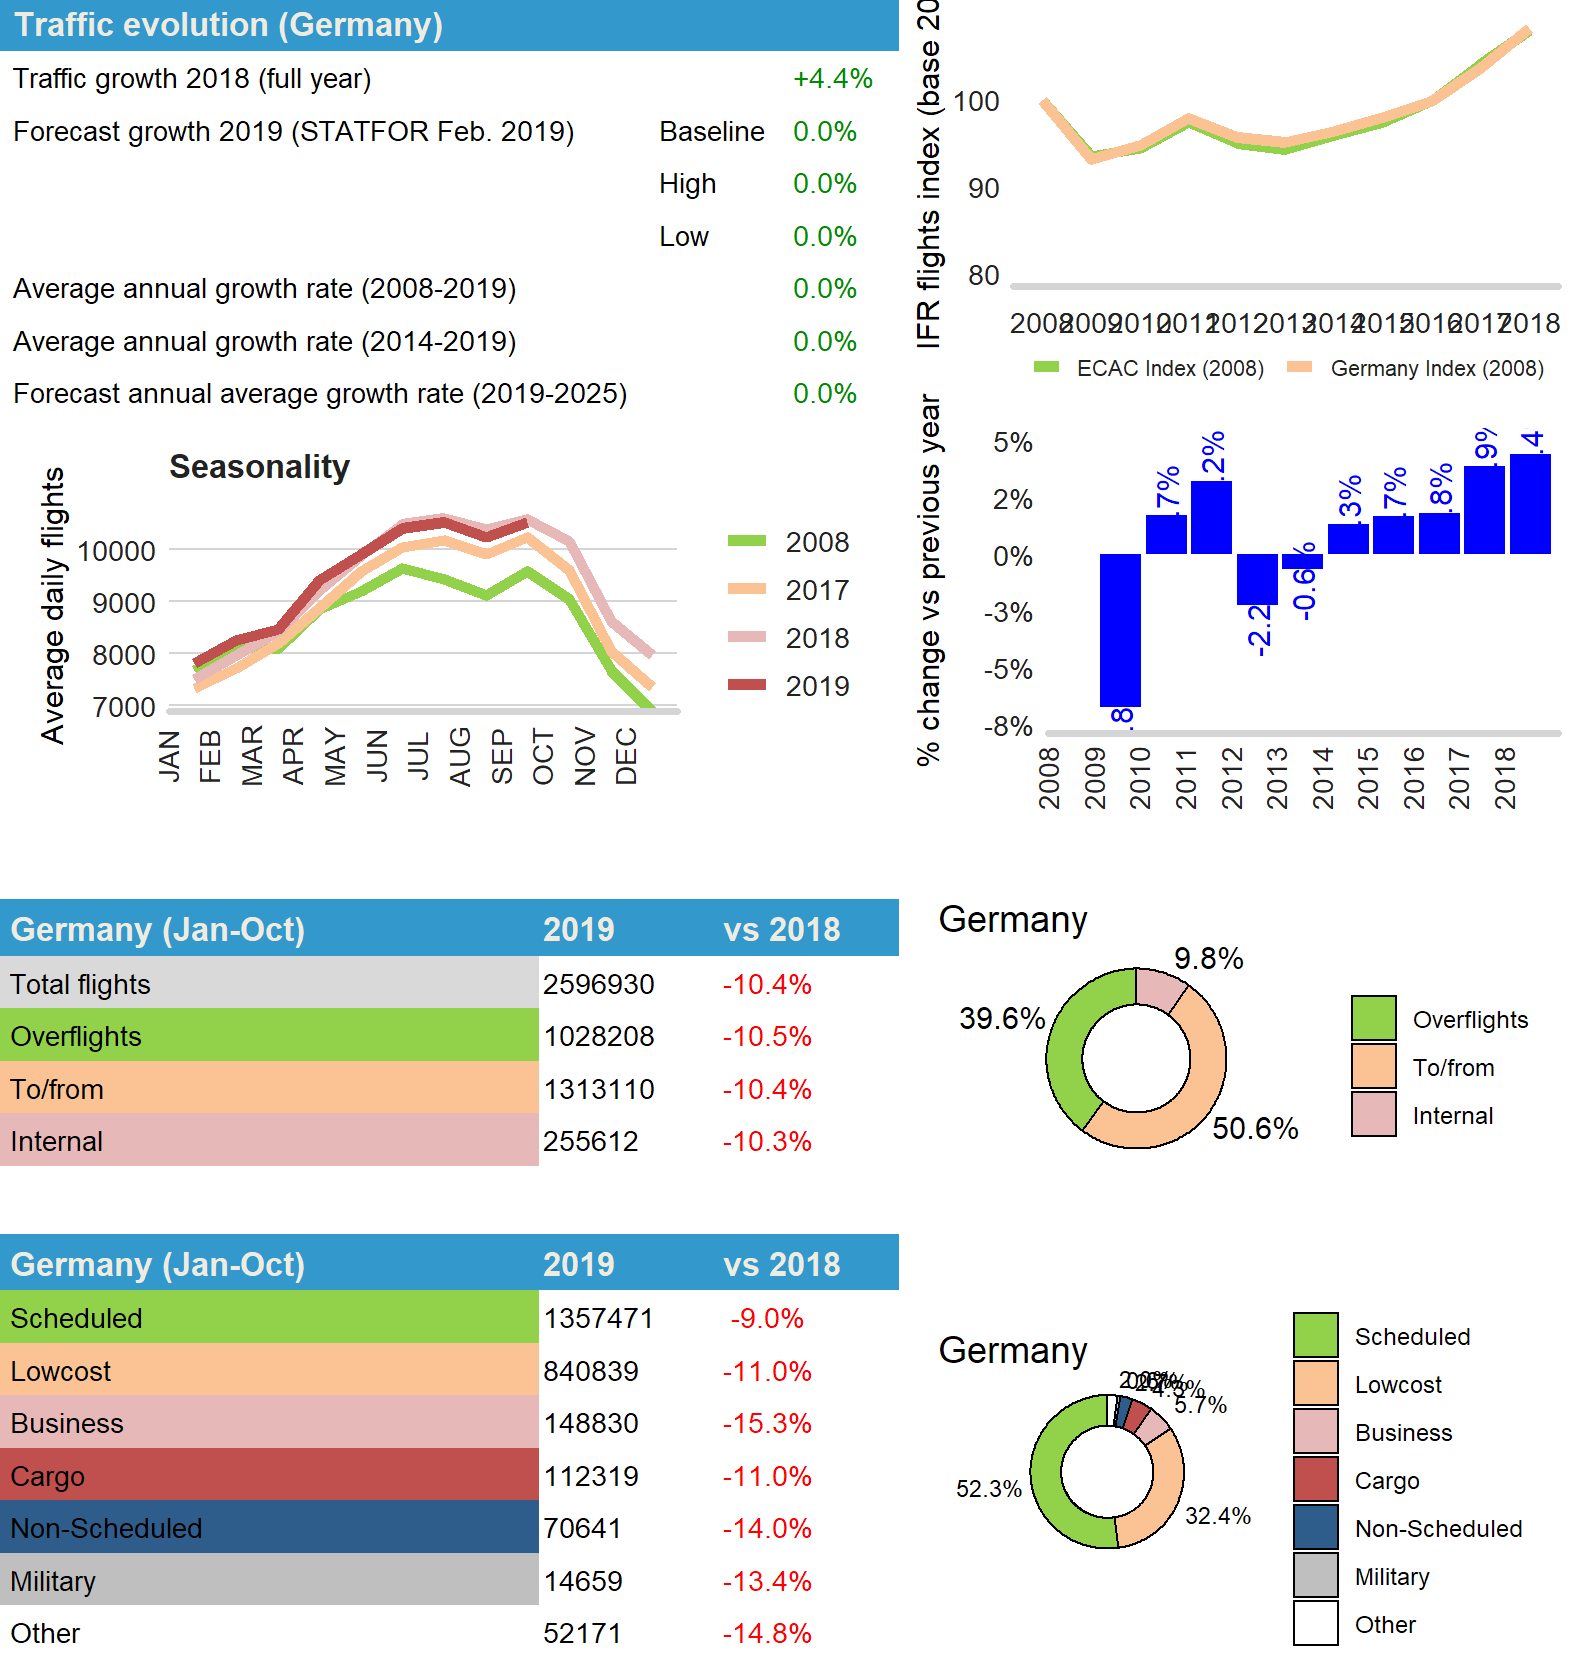
\includegraphics[width=\textwidth]{G:/HQ/dgof-pru/Project/Vertical_flight_efficiency/2015/State_briefing/Figures/Germany/Tfc_char_overview} 

}

\caption{Traffic characteristics (IFR flights)}(\#fig:Tfc-overview)
\end{figure}

\begin{itemize}
\tightlist
\item
  In 2018, traffic increased by +4.4\%. Between 2013 and 2018, traffic increased by 13.8\%.
\item
  In the first 11 months of 2019, traffic in Germany increased by +0.2\% compared to the same period in 2018
\item
  The largest traffic segment is traffic from and to Germany (50.7\%), followed by overflights (39.4\%) and domestic flights (9.9\%).
\end{itemize}

\newpage

\hypertarget{safety}{%
\section{Safety}\label{safety}}

\newpage

\hypertarget{capacity}{%
\section{Capacity}\label{capacity}}

\hypertarget{air-traffic-flow-management-atfm-delays}{%
\subsection{Air traffic flow management (ATFM) delays}\label{air-traffic-flow-management-atfm-delays}}

Source: NM, PRU ANS Performance Data Portal {[}\protect\hyperlink{ref-ANS-perf-data-portal}{3}{]}
The data in this section is from the PRU ANS performance data portal (data section).\\
It is available at: \url{http://ansperformance.eu/data/performancearea/}

\hypertarget{en-route-atfm-delays}{%
\subsubsection{En-route ATFM delays}\label{en-route-atfm-delays}}

\begin{figure}

{\centering 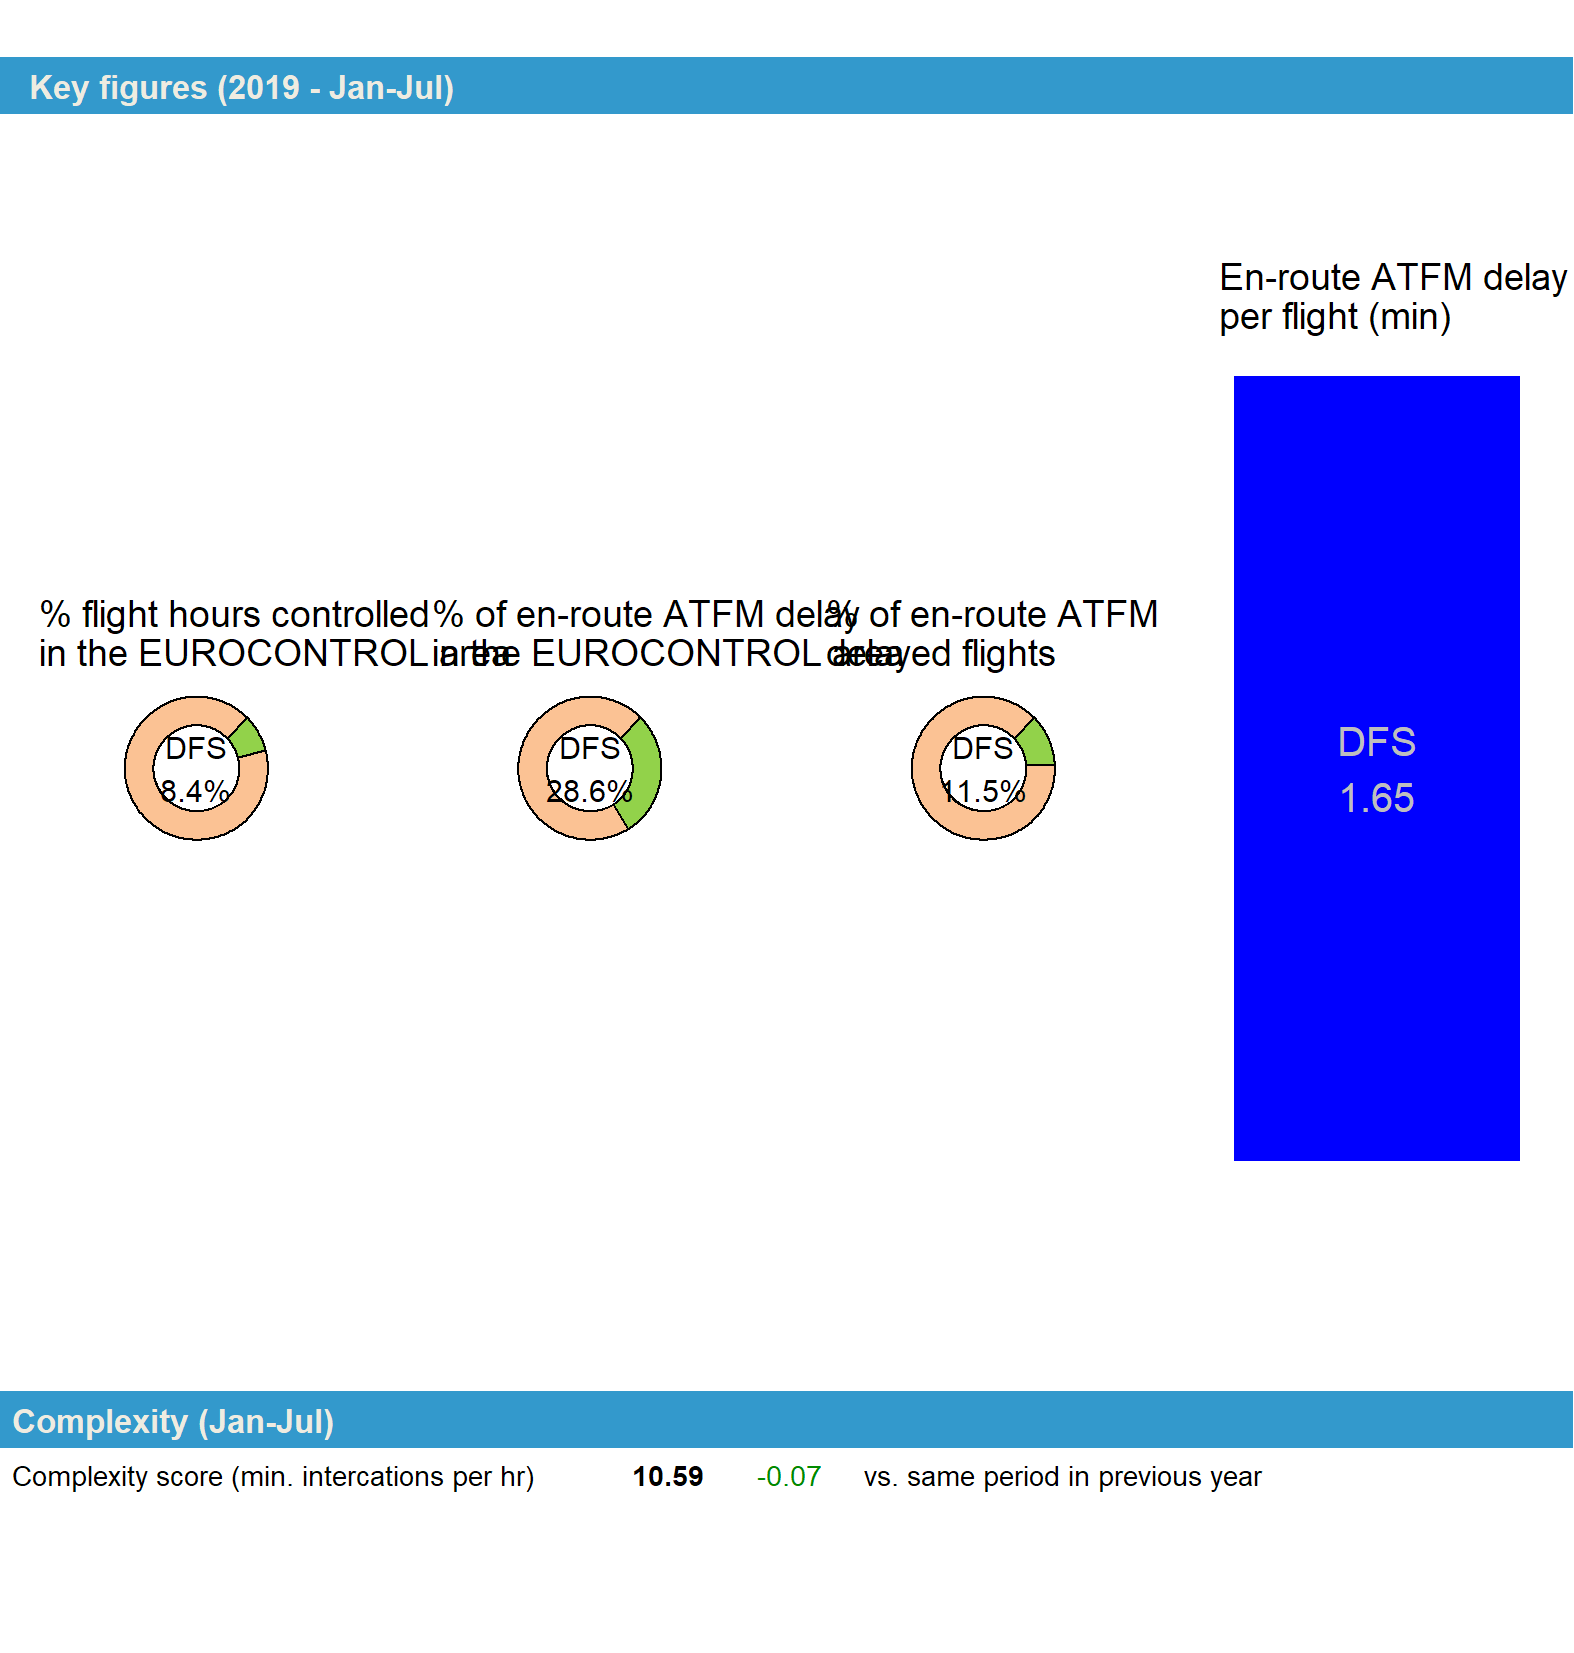
\includegraphics[width=\textwidth]{G:/HQ/dgof-pru/Project/Vertical_flight_efficiency/2015/State_briefing/Figures/Germany/ENR_capacity_overview} 

}

\caption{Traffic evolution and en-route ATFM delay}(\#fig:Capacity-overview)
\end{figure}

\begin{figure}

{\centering 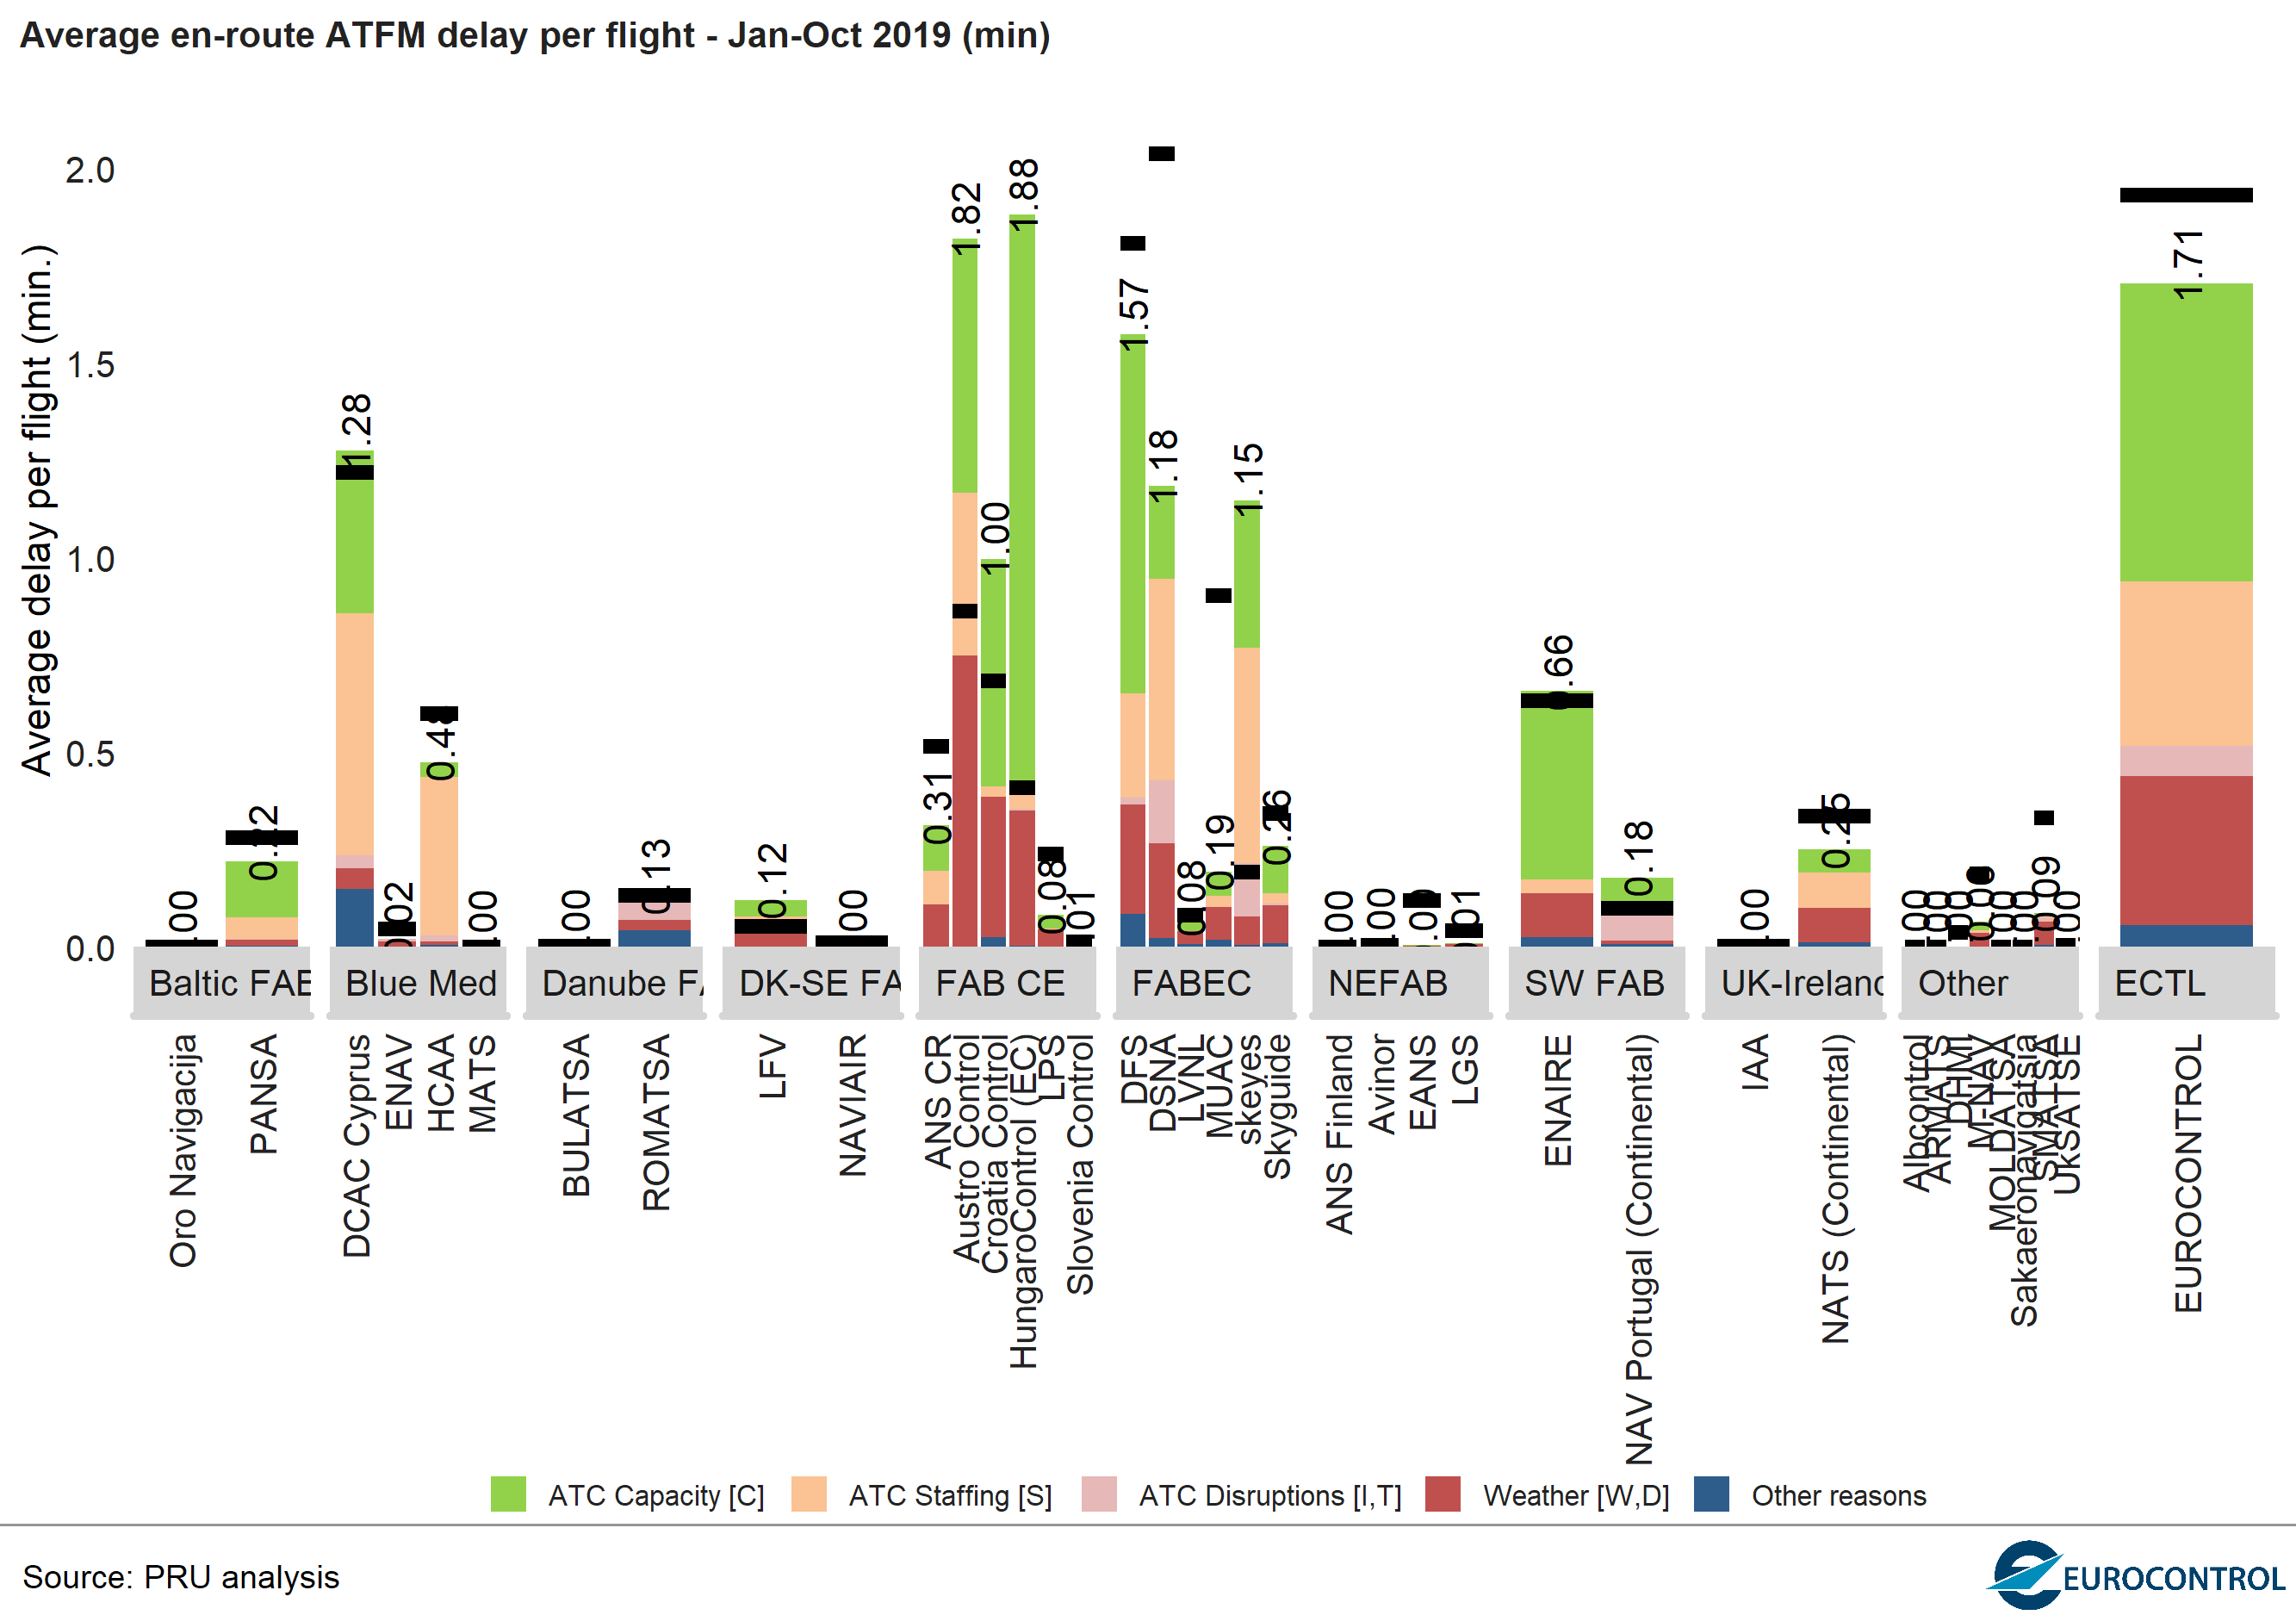
\includegraphics[width=\textwidth]{G:/HQ/dgof-pru/Project/Vertical_flight_efficiency/2015/State_briefing/Figures/Germany/ENR_delay_flight_bar} 

}

\caption{Average en route ATFM delay per flight (EUROCONTROL area)}(\#fig:AvgENR-ATFM-delay-flight)
\end{figure}

\begin{figure}

{\centering 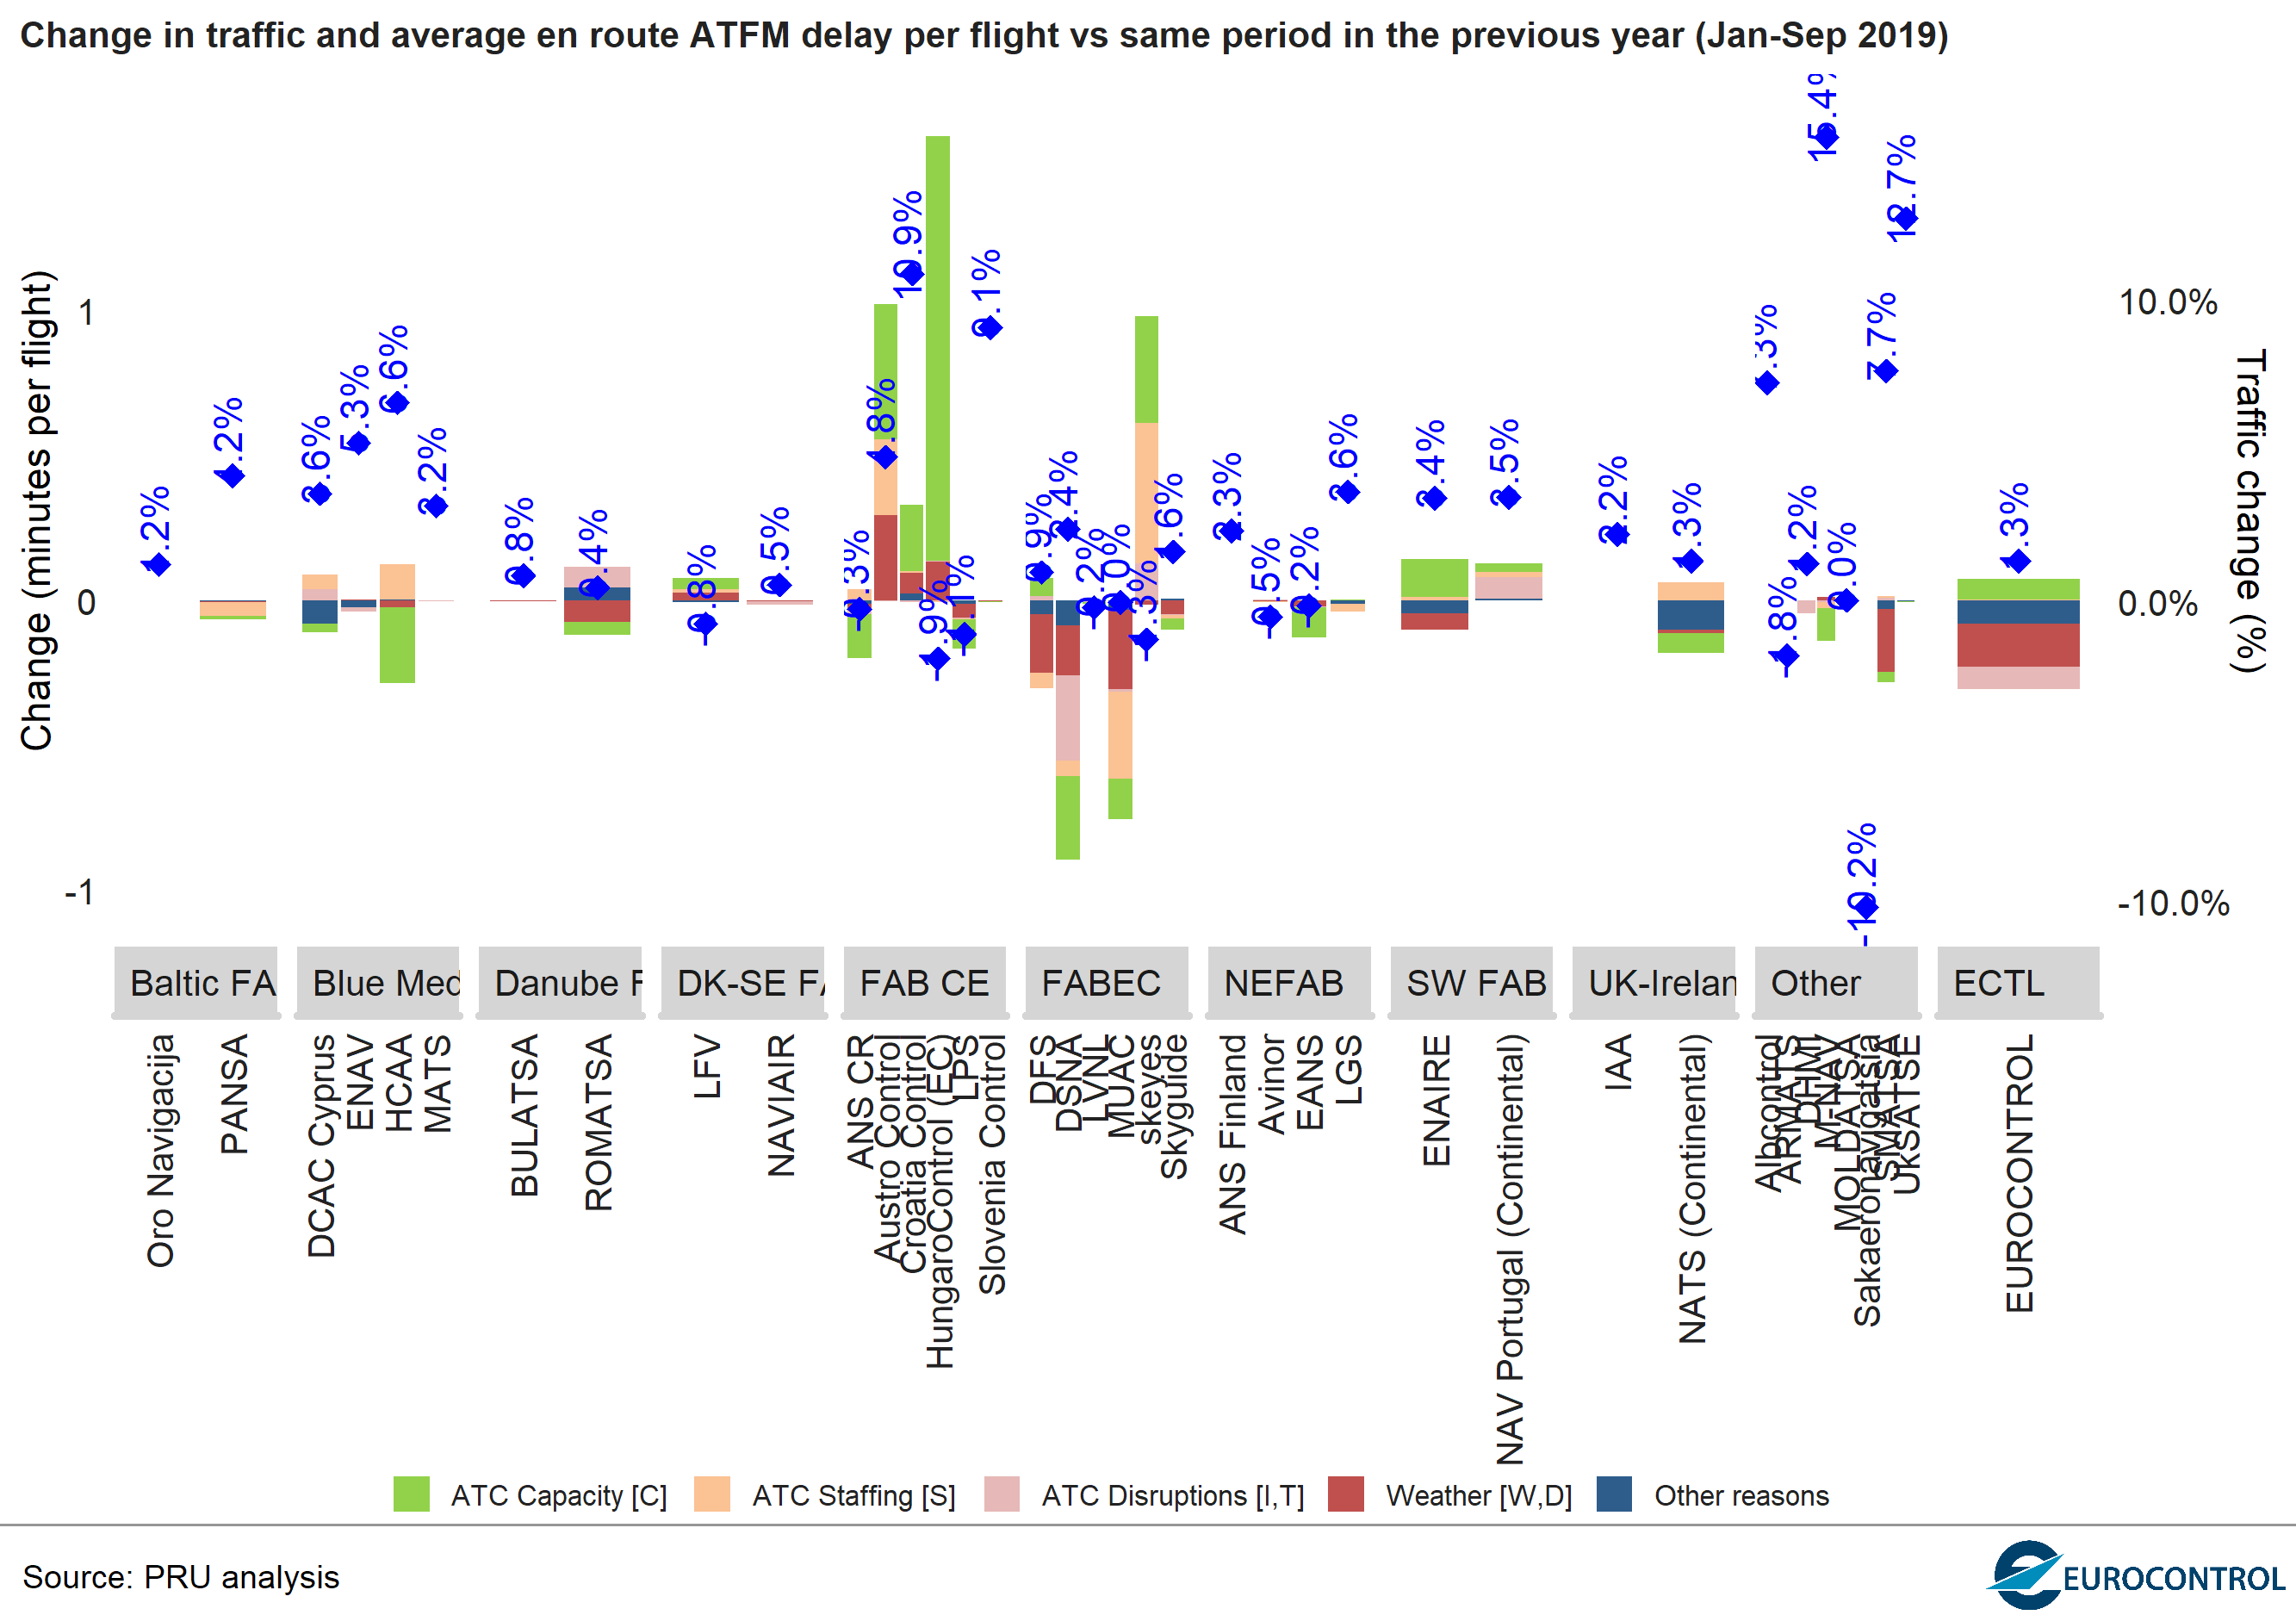
\includegraphics[width=\textwidth]{G:/HQ/dgof-pru/Project/Vertical_flight_efficiency/2015/State_briefing/Figures/Germany/ENR_delay_flight_change_bar} 

}

\caption{Year on year change of average en route ATFM delay per flight (EUROCONTROL area)}(\#fig:AvgENR-ATFM-delay-flight-change)
\end{figure}

\begin{itemize}
\tightlist
\item
  In the first 11 months of 2019, Germany accounted for 8.3\% of total controlled flight hours and generated 26.4\% of total en-route ATFM delays in the EUROCONTROL area. Overall, 10.8\% of the controlled flights in the respective airspace were delayed by en-route ATFM delays (Jan-Nov 2019).
\item
  Delays decreased in 2019 (-12.7\% vs.~Jan-Nov 2018) to reach 1.48 minutes per flight.
\end{itemize}

\hypertarget{airport-arrival-atfm-delays}{%
\subsubsection{Airport arrival ATFM delays}\label{airport-arrival-atfm-delays}}

\begin{figure}

{\centering 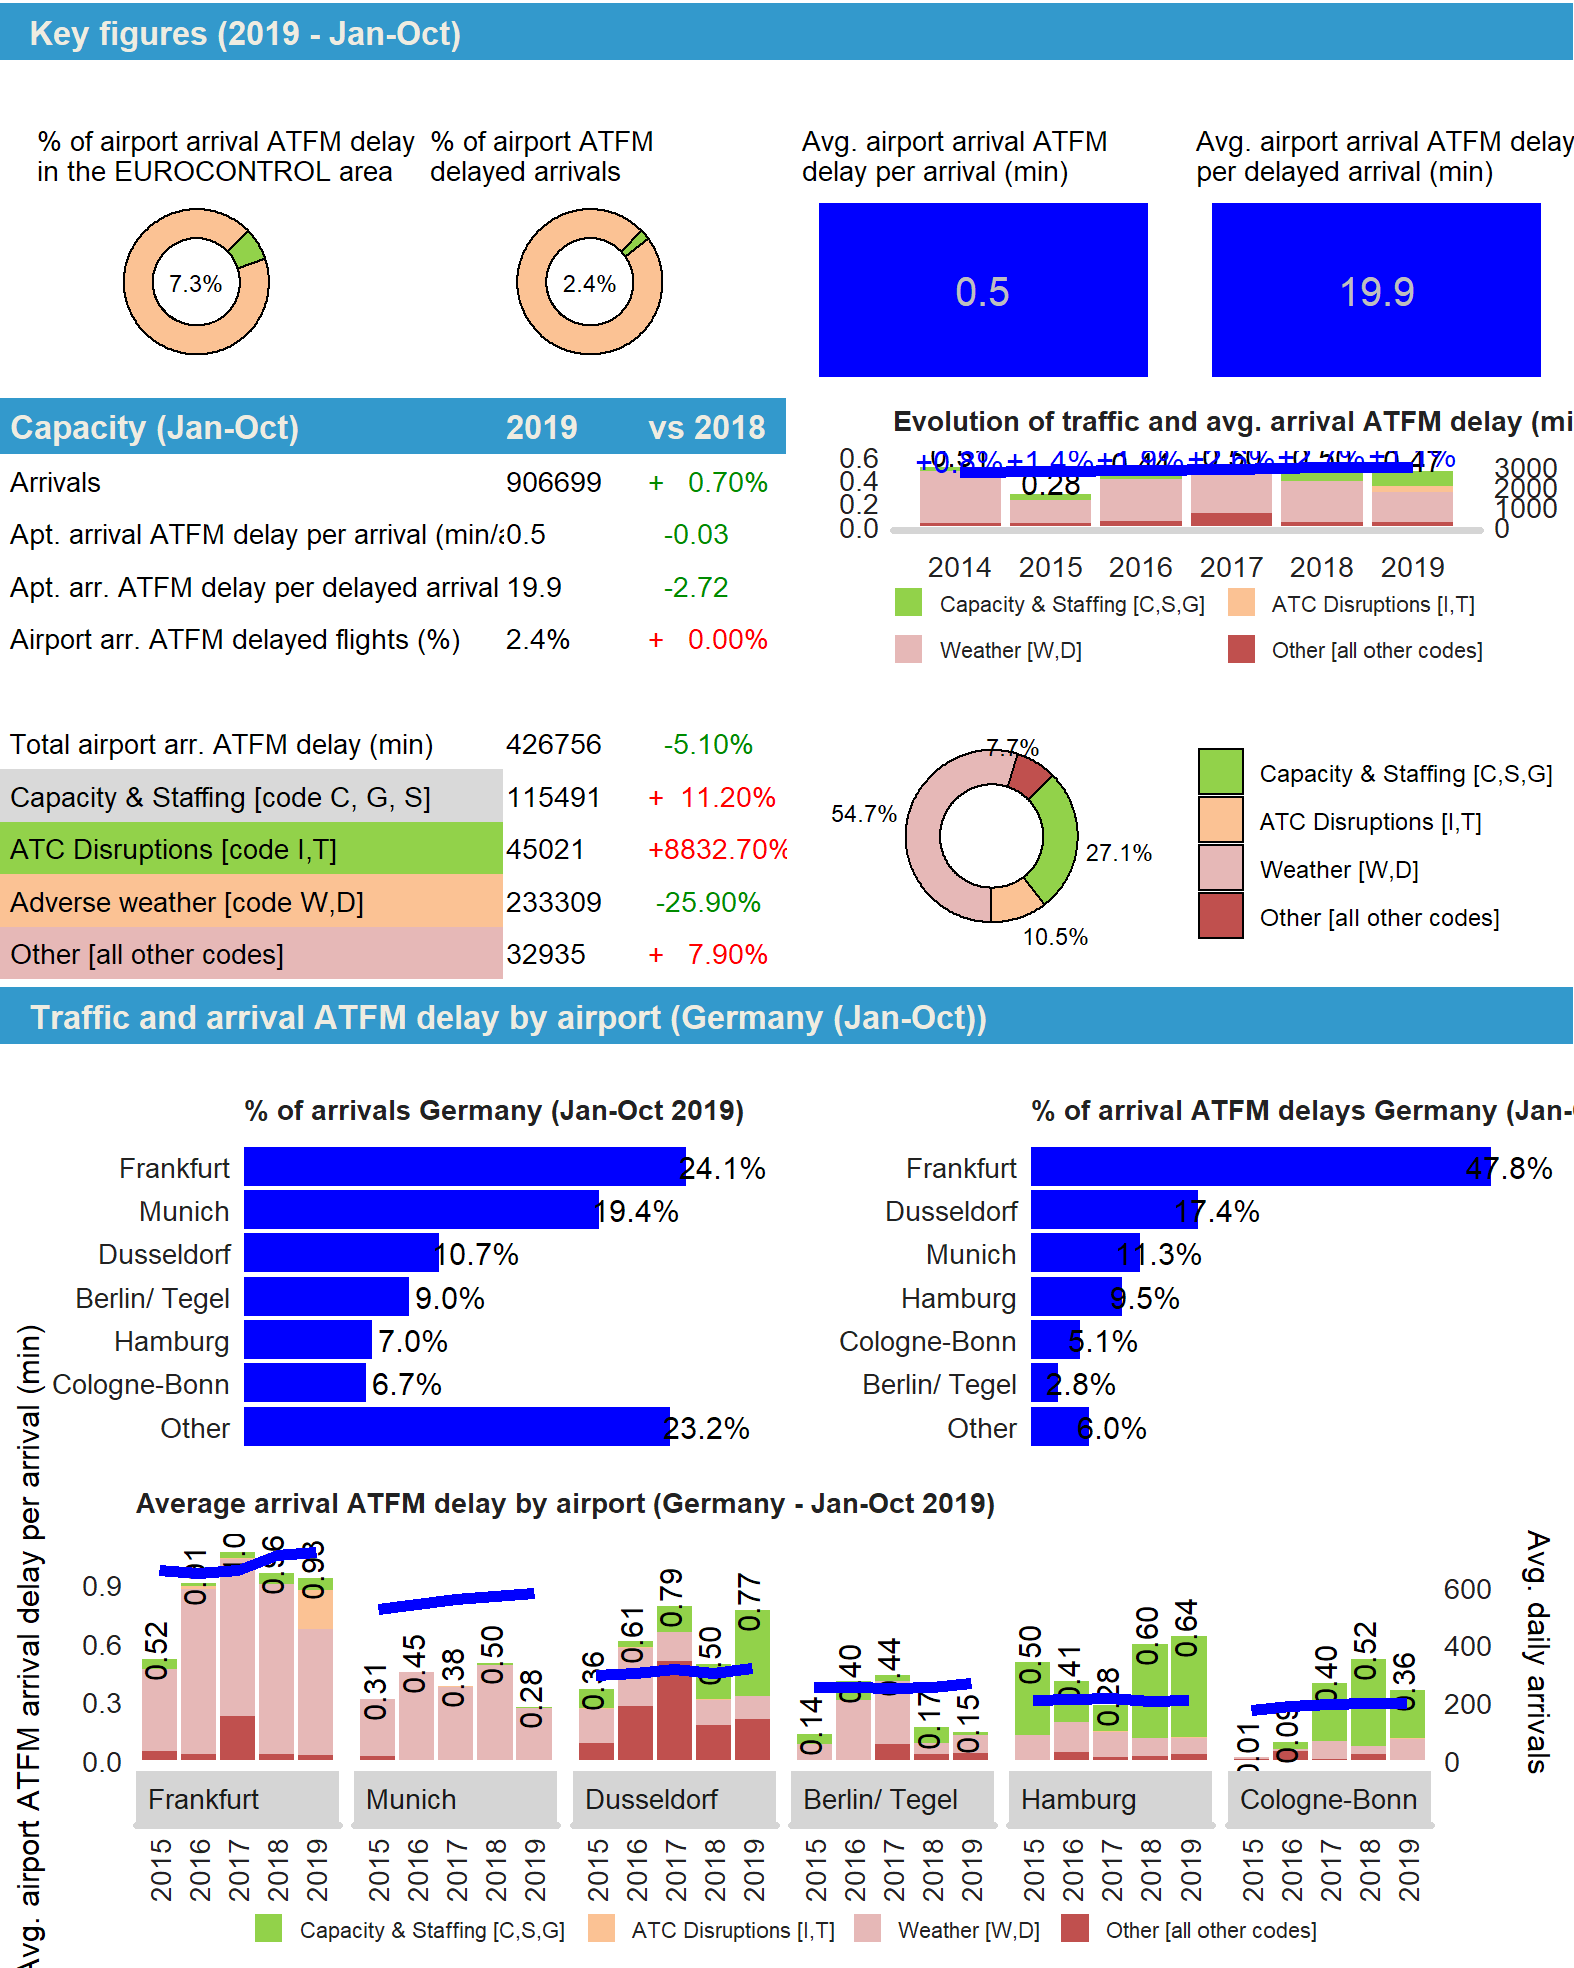
\includegraphics[width=\textwidth]{G:/HQ/dgof-pru/Project/Vertical_flight_efficiency/2015/State_briefing/Figures/Germany/APT_capacity_overview} 

}

\caption{Traffic evolution of airport arrival ATFM delays}(\#fig:Capacity-overview-APT)
\end{figure}

\begin{itemize}
\tightlist
\item
  Germany accounted for 7.4\% of all arrival ATFM delay in the EUROCONTROL area (Jan-Nov 2019).
\item
  Overall, 2.3\% of the flights arriving at airports in Germany were delayed by arrival ATFM regulations (Jan-Nov 2019). Total arrival ATFM delay decreased by -4.4\% vs.~Jan-Nov 2018.
\item
  The main share (47.9\%) was generated by Frankfurt, closely followed by Dusseldorf accounting for 16.9\% of all airport ATFM delay in Germany during the first 11 months of 2019.
\end{itemize}

\newpage

\hypertarget{environment}{%
\section{Environment}\label{environment}}

Source: PRU ANS Performance Data Portal
The data in this section is from the PRU ANS performance data portal (data section).\\
It is available at: \url{http://ansperformance.eu/data/performancearea/}

\hypertarget{horizontal-en-route-flight-efficiency}{%
\subsection{Horizontal en-route flight efficiency}\label{horizontal-en-route-flight-efficiency}}

\begin{figure}

{\centering 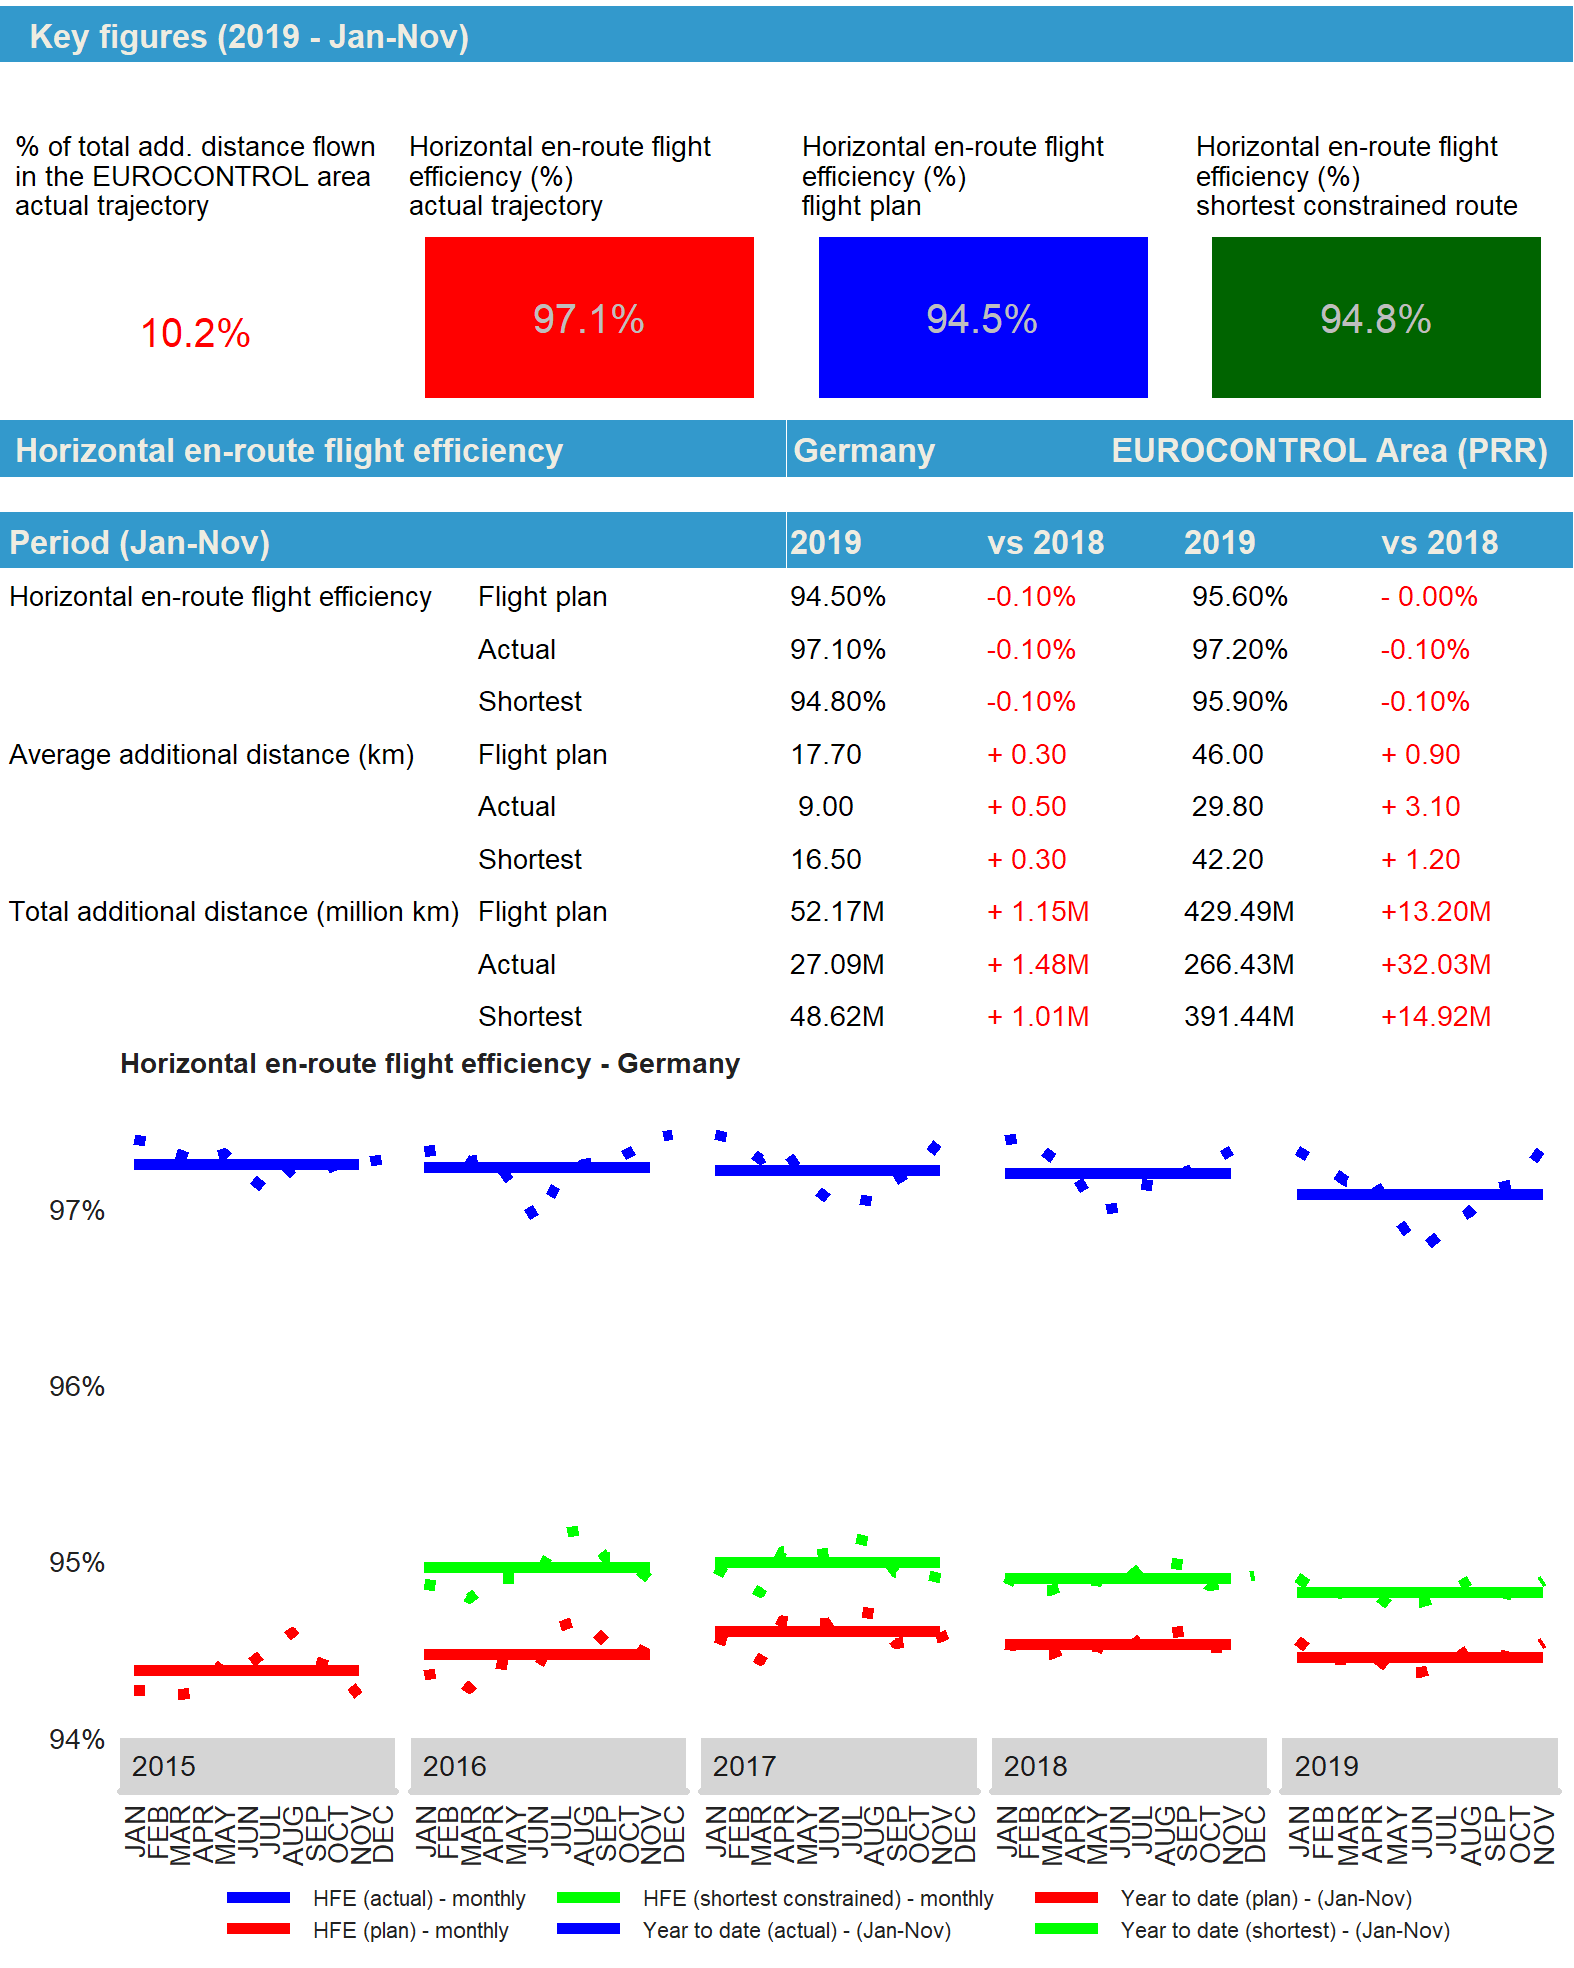
\includegraphics[width=\textwidth]{G:/HQ/dgof-pru/Project/Vertical_flight_efficiency/2015/State_briefing/Figures/Germany/HFE_overview} 

}

\caption{Horizontal en-route flight efficiency}(\#fig:HFE-overview)
\end{figure}

\begin{itemize}
\tightlist
\item
  Overall, Germany accounted for 10.2\% of the total additional distance flown in the EUROCONTROL area Jan-Nov 2019.
\item
  Horizontal en-route flight efficiency (actual trajectory) is 97.1\% which is below the EUROCONTROL area average (97.2\%).
\end{itemize}

\hypertarget{vertical-en-route-flight-efficiency}{%
\subsection{Vertical en-route flight efficiency}\label{vertical-en-route-flight-efficiency}}

\begin{figure}

{\centering 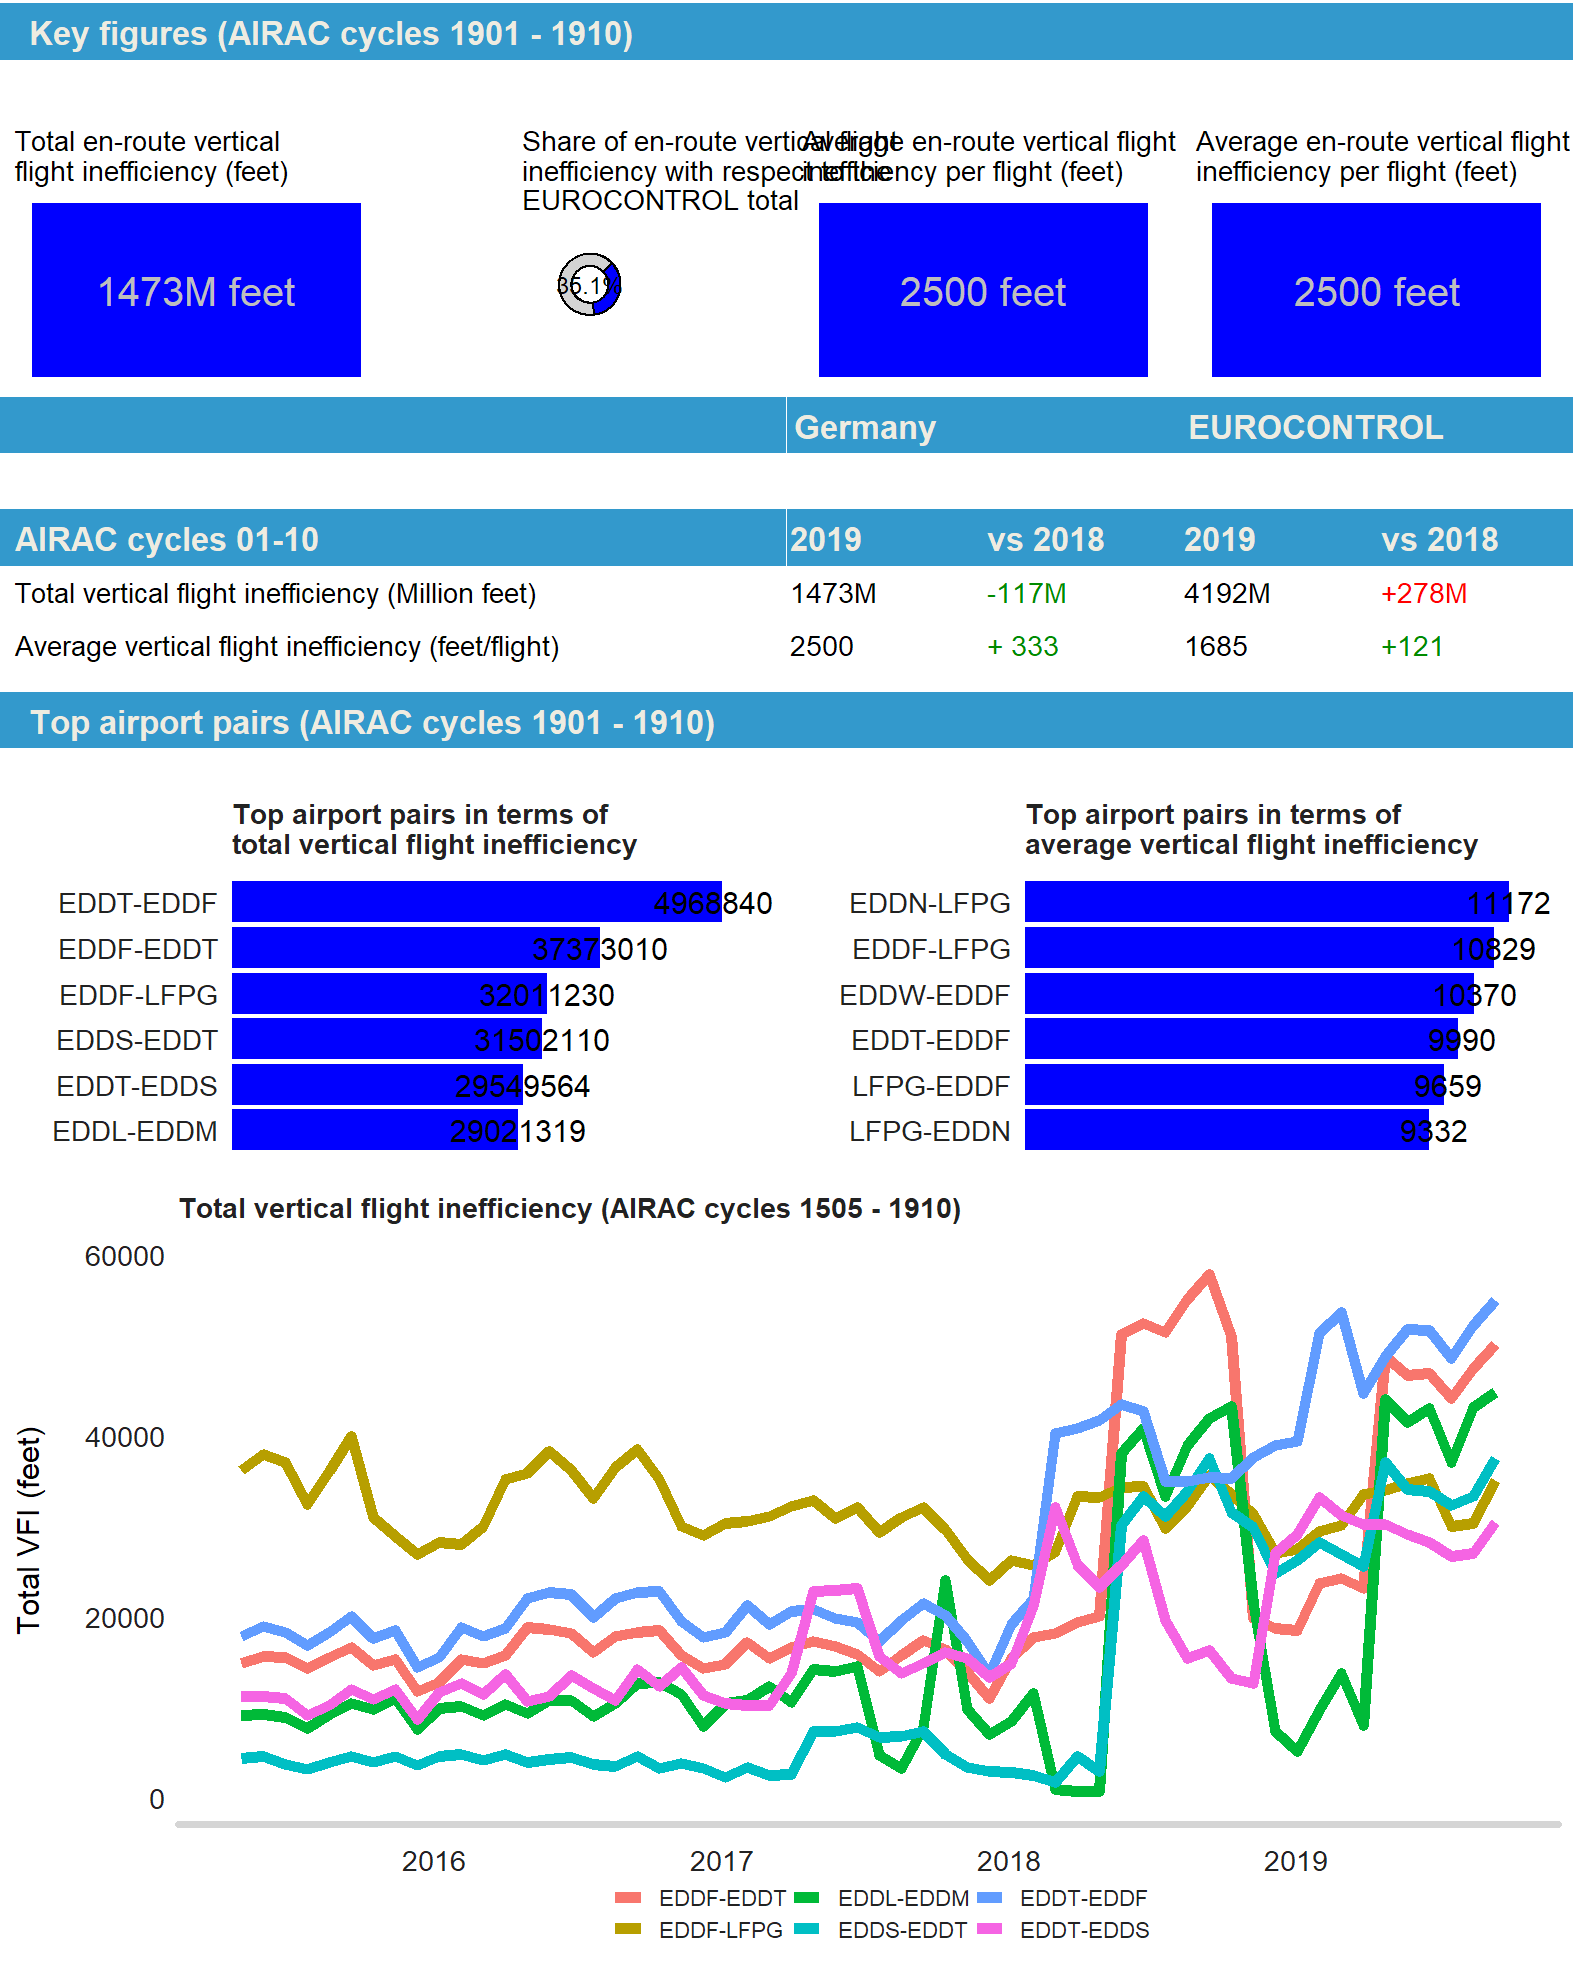
\includegraphics[width=\textwidth]{G:/HQ/dgof-pru/Project/Vertical_flight_efficiency/2015/State_briefing/Figures/Germany/ENR_VFE_overview} 

}

\caption{Vertical en-route flight efficiency}(\#fig:ENR-VFE-overview)
\end{figure}

\hypertarget{vertical-flight-efficiency-during-climb-descent}{%
\subsection{Vertical flight efficiency during climb \& descent}\label{vertical-flight-efficiency-during-climb-descent}}

\begin{figure}

{\centering 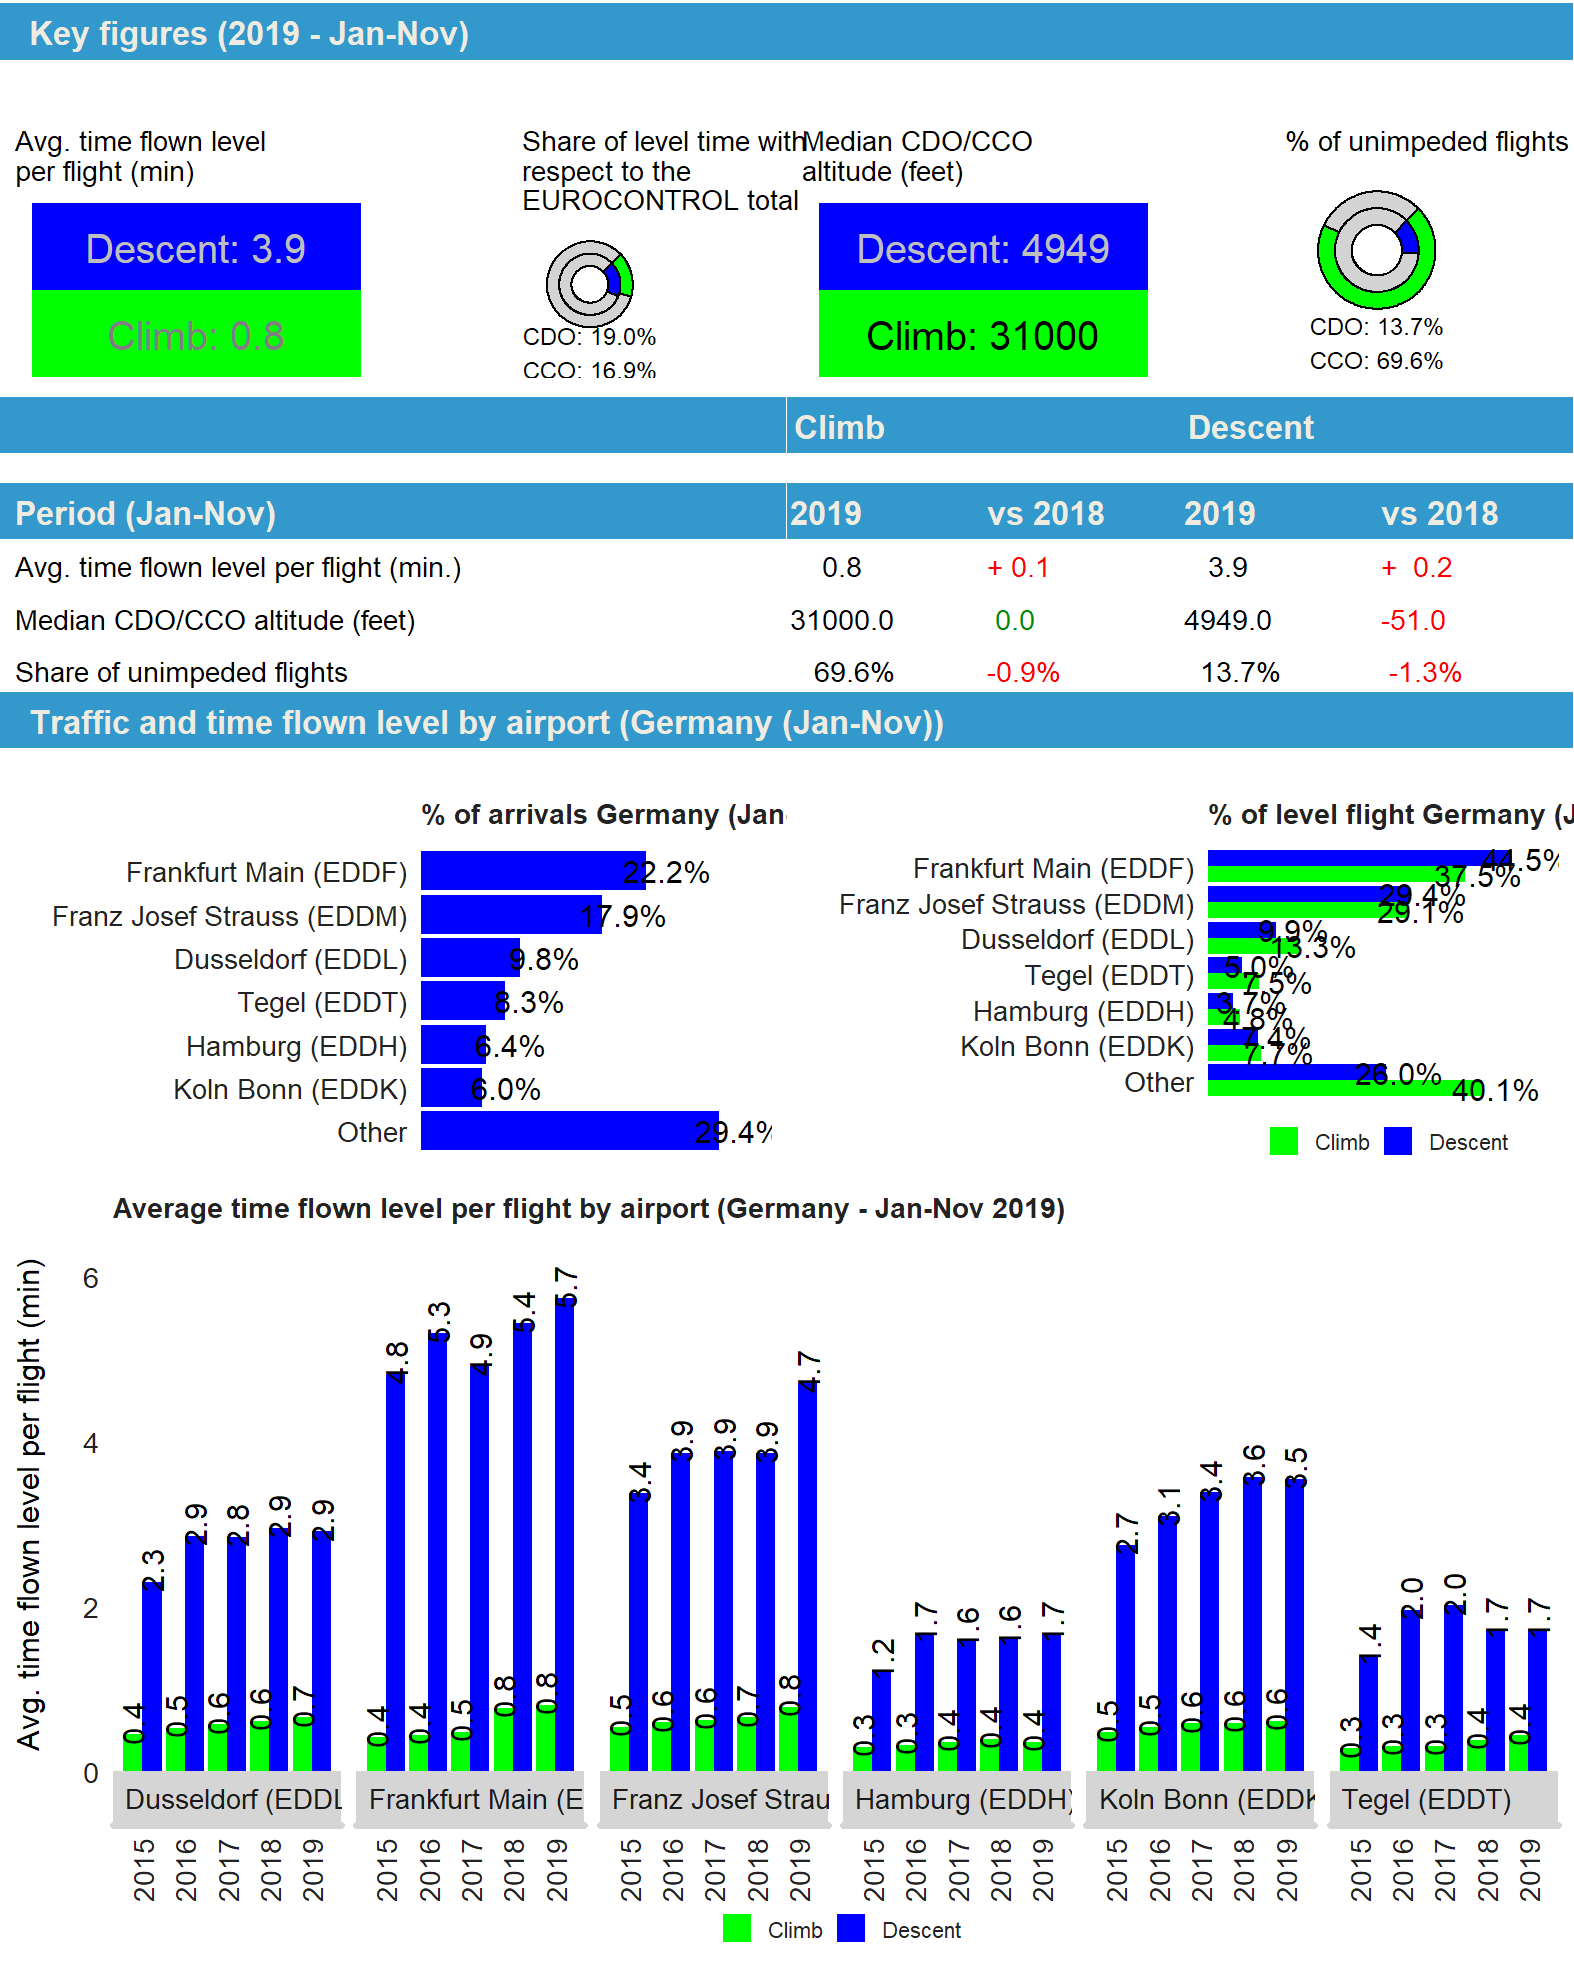
\includegraphics[width=\textwidth]{G:/HQ/dgof-pru/Project/Vertical_flight_efficiency/2015/State_briefing/Figures/Germany/CDO_CCO_overview} 

}

\caption{Vertical flight efficiency during climb and descent}(\#fig:CDO-CCO-overview)
\end{figure}

\newpage

\hypertarget{cost-effectiveness}{%
\section{Cost-effectiveness}\label{cost-effectiveness}}

\newpage

\hypertarget{annex-1-evolution-of-cost-effectiveness-performance-2012-2017}{%
\section{Annex 1: Evolution of cost-effectiveness performance (2012-2017)}\label{annex-1-evolution-of-cost-effectiveness-performance-2012-2017}}

\newpage

\hypertarget{annex-2-network-operations-plan-2018-201922}{%
\section{Annex 2: Network Operations Plan (2018-2019/22)}\label{annex-2-network-operations-plan-2018-201922}}

\newpage

\hypertarget{references}{%
\section*{References}\label{references}}
\addcontentsline{toc}{section}{References}

\hypertarget{refs}{}
\leavevmode\hypertarget{ref-pru:ace-report-2015}{}%
{[}1{]} Performance Review Unit, ``ATM cost-effectiveness (ace) 2015 benchmarking report with 2016-2020 outlook,'' EUROCONTROL/PRU, Report, May 2017.

\leavevmode\hypertarget{ref-7year-forecast-2019}{}%
{[}2{]} STATFOR, ``EUROCONTROL seven-year forecast february 2019,'' EUROCONTROL/STATFOR, Report, 2017.

\leavevmode\hypertarget{ref-ANS-perf-data-portal}{}%
{[}3{]} Performance Review Unit, ``ANS performance data portal,'' 2019. {[}Online{]}. Available: \url{http://ansperformance.eu/}.

\leavevmode\hypertarget{ref-service-unit-dashboard}{}%
{[}4{]} CRCO, ``Service unit dashboard,'' 2019. {[}Online{]}. Available: \url{http://www.eurocontrol.int/ServiceUnits/Dashboard/LongTermEvolution.html}.

\end{document}
